\thispagestyle{empty}
\vspace{3.0ex}
\begin{center}\uppercase{\normalsize Siglen, Abkürzungen, Zeichen}\end{center}
\vspace{4.0ex}% PR: Rein provisorisch!
\renewcommand*{\chapter}{\OrigChapter}
\noindent\footnotesize
\uppercase{1. Siglen und editorische Zeichen}\\[3.0ex]
\begin{tabular}{lp{110mm}}
\textit{A} & fremdhändige Abschrift eines fremden Textes\\
\textit{E}, \textit{E}\textsuperscript{1} & Erstdruck\\
\textit{E}\textsuperscript{2} ... & weitere Drucke\\
\textit{L}, \textit{L\textsuperscript{1}} ... & Leibniz, eigenhändig\\
\textit{l} & Leibniz, Abschrift von Schreiberhand\\
 \textit{LiA} & Leibnizens eigenhändige Bemerkungen und Verbesserungen in einer fremdhändigen Abschrift eines fremden Textes\\
\textit{Lil} & Leibnizens eigenhändige Bemerkungen und Verbesserungen in einer Abschrift von Schreiberhand\\
%\textit{LiH} & Leibniz' eigenhändige Anstreichungen und Anmerkungen in einem Handexemplar\\
\textit{Ü} & Übersetzung\\
\lbrack~\rbrack& bei Datierungen: erschlossenes Datum
\newline im Text und bei Abbildungen: Änderungen, Ergänzungen und Erläuterungen des Herausgebers
\newline von Leibniz benutzte eckige Klammern werden im Erläuterungs\-apparat angezeigt\\
\lbrack/\rbrack&Zeilenfall in diplomatisch wiedergegebenem Text %
oder im Stufenapparat
\\
\lbrack...\rbrack &im Stufenapparat: Gültiger Text, der im Haupttext vollständig wiedergegeben wird\\
\lbrack\textit{!}\rbrack &im Stufenapparat: nicht verbesserte Rechen- oder Sprachfehler\\ %MS
% \textit{[~]} & vom Herausgeber hinzugefügte Figurenbezeichnungen\\
% \textit{(~)} & von Leibniz in Figuren seines Handexemplars hinzugefügte Bezeichnungen\\
$\langle$\ $\rangle$ & Konjektur schwer lesbarer oder durch Beschädigung der Handschrift ausgefallener Wörter bzw. Wortteile\\
$\langle$...$\rangle$ $\langle$\textendash $\rangle$~$\langle$\textendash~\textendash$\rangle$& nicht entzifferter bzw. durch Beschädigung der Handschrift aus\-gefallener Text unbestimmter Länge oder im Umfang vermutlich eines oder mehrerer Worte\\
\textit{Kursivierung} &zitierter Titel von Büchern oder Schriften
\newline wörtliches oder fast wörtliches Zitat;
als \glqq fast wörtlich\grqq\ gilt eine Text\-wiedergabe, die unbedeutsam von der Vorlage abweicht,
etwa bei flüchtiger Wortfolge oder Kasus\-änderungen\\
% ??Text in anderer als der Grundsprache des betreffenden Textes
% \newline ??Herausgebertext\\
\textso{Sperrung} & Hervorhebungen durch Leibniz %Die Art der Hervorhebung wird im Er\-läuterungsapparat angezeigt.
\end{tabular}
\vspace{4.0ex}
%%%%
%%%%

\noindent\footnotesize
\uppercase{2. Abkürzungen} (allgemein)
\setlength\LTleft{0pt} \setlength\LTright{0pt}
\begin{longtable}{ll}
a.a.O. & am angegebenen Ort\\
Anm. & Anmerkung\\
Aufl. & Auflage\\
Bd(e) & Band (Bände)\\
bes. & besonders\\
Bl. & Blatt\\
bspw. & beispielsweise\\
bzw.  & beziehungsweise\\
c. & caput (capita), capitulum (capitula)\\
ca. & circa\\
cap. & caput (capita), capitulum (capitula)\\
chap. & chapitre(s)\\
d.h. & das heißt\\
ebd. & ebenda\\
e.g. & exempli gratia\\
eigh. & eigenhändig\\
erg. & ergänzt\\
Erl. & Erläuterung\\
f. (ff.) & folgend(e)\\
Fig. & Figur\\
fl. & floruit\\
fol. & folio\\
gestr. & gestrichen\\
GWLB & Gottfried Wilhelm Leibniz Bibliothek \textendash\ Niedersächsische Landesbibliothek\\
H. & Hälfte\\
Hrsg. (hrsg.) & Herausgeber (herausgegeben)\\
Hs. & Handschrift\\
Jh. & Jahrhundert\\
% KAT & Arbeitskatalog der Leibniz-Edition (\glqq Ritter-Katalog\grqq)\\
% k.E. & kein Eintrag\\
l. & liber (libri)\\
LBr & \textsc{Hannover}, GWLB, Leibniz-Briefwechsel\\
LH & \textsc{Hannover}, GWLB, Leibniz-Handschriften\\
lib. & liber (libri)\\
m. & mit\\
Marg. & Marginalie(n)\\
Ms. & Manuskript\\
n. & numerus (numeri)\\
N. & Stücknummer(n) in der \textit{LSB}-Ausgabe\\
Nachdr. & Nachdruck\\
NB & nota bene\\
Nr. & Nummer(n)\\
o.S. & ohne Seitenangabe\\
p. & pagina(e), page(s)\\
r\textsuperscript{o} & recto\\
% RS & Royal Society\\
S. & Seite(n)\\
Sp. & Spalte(n)\\
%SV & Schriftenverzeichnis\\
% TD & Teildruck\\
tlw. & teilweise\\
u. & und\\
u.a. & und andere, unter anderem\\
u.ö. & und öfters\\
v. & van, von\\
v.c. & verbi causa\\
v.g. & verbi gratia\\
vgl. & vergleiche\\
% vermutl. & vermutlich\\
v\textsuperscript{o} & verso\\
Z. & Zeile(n)\\
z.B. & zum Beispiel
\end{longtable}
\vspace{3.0ex}
%\clearpage
\noindent\footnotesize{\uppercase{3. Abkürzungen} (Schriften)}\par
\vspace{2.0ex}
%%%%
%%%%

%\setlength\LTleft{0pt} \setlength\LTright{0pt}
%\begin{longtable}{lp{105mm}}
\noindent\hangindent=10mm\textit{AE:} \textit{Acta Eruditorum}, hrsg.\ von O.~Mencke und J.\,B.~Mencke,
50 Bde, Leipzig 1682\textendash 1731.\par
%
\noindent\hangindent=10mm\textsc{Antognazza} 2009: M.~R.\ \textsc{Antognazza} \textit{Leibniz. An Intellectual Biography}, Cambridge (UK) 2009.\par
%
\noindent\hangindent=10mm\textsc{Bertoloni Meli} 1993: D.\ \textsc{Bertoloni Meli}, \textit{Equivalence and Priority: Newton versus Leibniz. Including Leibniz's Unpublished Manuscripts on the Principia}, Oxford 1993.\par
%
%\noindent\hangindent=10mm\textit{BH:} T.\ \textsc{Birch}, \textit{The History of the Royal Society of London for improving of natural knowledge: from its first rise}, London 1757.\par
%
%\noindent\hangindent=10mm\textit{BW:} R.\ \textsc{Boyle}, \textit{The Works}, hrsg.\ von M.~Hunter und E.\,B. Davis, 14 Bde, London 1999\textendash2000.\par
%
\noindent\hangindent=10mm Cc 2: \textit{Catalogue critique des manuscrits de Leibniz, Fascicule  II (Mars 1672\textendash Novembre 1676)}, hrsg.\ von A.~Rivaud u.a., Poitiers 1914\textendash 1924.\par
%
\noindent\hangindent=10mm\textit{Chronik:} \textit{Leben und Werk von Gottfried Wilhelm Leibniz: Eine Chronik}, bearb.\ von K.~Müller und G.~Krönert, Frankfurt am Main 1969.\par
%
\noindent\hangindent=10mm\textit{DL:} R.\ \textsc{Descartes}, \textit{Lettres de M.~Descartes}, hrsg.\ von C.~de Clerselier, 3 Bde, Paris 1657\textendash 1667.\par
%
\noindent\hangindent=10mm\textit{DO:} R.\ \textsc{Descartes}, \textit{Oeuvres}, hrsg.\ von C.~Adam und P.~Tannery, 12 Bde, Paris 1879\textendash 1910, 2.~Aufl.\ ebd.\ 1964\textendash 1972.\par
%
\noindent\hangindent=10mm\textsc{Fichant} 1994: G.\,W. \textsc{Leibniz}, \textit{La réforme de la dynamique. De corporum concursu (1678) et autres textes inédits}, hrsg.\ von M.~Fichant, Paris 1994.\par
%
\noindent\hangindent=10mm\textsc{Gerland} 1906: G.\,W. \textsc{Leibniz}, \textit{Nachgelassene Schriften physikalischen, mechanischen und technischen Inhalts}, hrsg.\ von E.~Gerland, Leipzig 1906; Nachdr.\ Hildesheim, New York 1995.\par
%
\noindent\hangindent=10mm\textit{GO:} G.\ \textsc{Galilei}, \textit{Opere. Edizione Nazionale}, hrsg.\ von A.~Favaro u.a., 20 Bde, Florenz 1890\textendash 1909.\par
%
\noindent\hangindent=10mm\textit{GOO:} P.\ \textsc{Gassendi}, \textit{Opera omnia}, 6 Bde, Lyon 1658; Nachdr.\ Stuttgart-Bad Cannstatt 1964.\par
%
\noindent\hangindent=10mm\textit{HO:} C.\ \textsc{Huygens}, \textit{Oeuvres compl\`{e}tes}, hrsg.\ von D.~Bierens de Haan, J.~Bosscha u.a., 22 Bde, Den Haag 1888\textendash 1950.\par
%
\noindent\hangindent=10mm\textit{JS:} \textit{Journal des S\c{c}avans}, Paris 1665ff.\par
%
\noindent\hangindent=10mm\textit{KGW:} J.\ \textsc{Kepler}, \textit{Gesammelte Werke}, hrsg.\ von der Bayerischen Akademie der Wissenschaften, 27 Bde, München %
1937\textendash2017.\par
%
%\noindent\hangindent=10mm KK 1: \textit{Kritischer Katalog der Leibniz-Handschriften, 1.\ Heft 1646\textendash 1672}, hrsg.\ von P.~Ritter, als Manuskript veröffentlicht Berlin 1908.\par
%
\noindent\hangindent=10mm\textsc{Lamarra/Palaia} 2005: G.\,W.\ \textsc{Leibniz}, \textit{Essais scientifiques et philosophiques}, hrsg.\ von A.~Lamarra und R.~Palaia, 3 Bde, Hildesheim, Zürich, New York 2005.\par
%
\noindent\hangindent=10mm\textit{LMG:} \textit{Leibnizens gesammelte Werke}, hrsg.\ von G.\,H.~Pertz, Dritte Folge: Mathematische Schriften, hrsg.\ von C.\,I.~Gerhardt, 7 Bde, Berlin, Halle 1849\textendash 1863; Nachdr.\ Hildesheim 1971.\par
%
\noindent\hangindent=10mm\textit{LOD}: G.\,W.\ \textsc{Leibniz}, \title{Opera omnia}, hrsg.\ von L.~Dutens, 6 Bde, Genf 1768; Nachdr.\ Hildesheim 1990.\par
% \noindent\hangindent=10mm\textsc{Dutens}: \textsc{Leibniz, G. W.}, \textit{Opera omnia, nunc primum collecta, in classes distributa, praefationibus et indicibus exornata}, hrsg.\ von L.~Dutens, 6 Bde, Genf 1768; Nachdr.\ Hildesheim 1990.\par
%
\noindent\hangindent=10mm\textit{LPG:} \textit{Die philosophischen Schriften von Gottfried Wilhelm Leibniz}, hrsg.\ von C.\,I.~Gerhardt, 7 Bde, Berlin 1875\textendash 1890; Nachdr.\ Hildesheim 1996.\par
%
\noindent\hangindent=10mm\textit{LSB:} G.\,W.\ \textsc{Leibniz}, \textit{Sämtliche Schriften und Briefe}, Akademie-Ausgabe, Darmstadt 1923ff.\
(seit 1954: Berlin).\par
%
\noindent\hangindent=10mm\textit{MO:} E.\ \textsc{Mariotte}, \textit{Oeuvres, comprenant tous le Traitez de cet Auteur, tant ceux qui avoient déja paru séparément, que ceux qui n'avoient pas encore été publiez}, 2 Bde, Leiden 1717.\par
%
\noindent\hangindent=10mm\textit{PO:} B.\ \textsc{Pascal}, \textit{Oeuvres}, hrsg.\ von P.~Boutroux, L.~Brunschvicg und F.~Gazier, 14~Bde, Paris 1904\textendash 1914; Nachdr.\ Vaduz 1965.\par
%
\noindent\hangindent=10mm\textit{PT:} %
\textit{Philosophical Transactions of the Royal Society}, London 1665ff.\par
%
% \noindent\hangindent=10mm\textit{SPW}: S.\ \textsc{Stevin}, \textit{The principal works}, hrsg.\ von E.\,J.~Dijksterhuis u.a., Amsterdam 1955\textendash 1966.\par
%
\noindent\hangindent=10mm\textit{SVF:}
\textit{Stoicorum veterum fragmenta}, hrsg.\ von H.~von~Arnim (Bd IV mit M.\,Adler), 4 Bde, Leipzig 1903\textendash 1924.\par
%
%\noindent\hangindent=10mm\textit{TBO:} T.\ \textsc{Brahe}, \textit{%Tychonis Brahe Dani 
%Opera omnia}, hrsg.\ von J.\,L.\,E.~Dreyer, 15 Bde, Kopenhagen 1913\textendash 1929.\par
%
\noindent\hangindent=10mm\textit{TO:} E.\ \textsc{Torricelli}, \textit{Opere}, hrsg.\ von G.~Loria und G.~Vassura, 4 Bde, Faenza 1919\textendash 1944.\par
%
\noindent\hangindent=10mm\textit{WO:} J.\ \textsc{Wallis}, \textit{Opera mathematica}, 3 Bde, Oxford 1693\textendash 1699; Nachdr.\ Hildesheim 1972.\par
%
%\end{longtable}
\vspace{6.0ex}
%%%%

\newpage

\noindent\footnotesize{\uppercase{4. Symbole}}
\setlength\LTleft{0pt} \setlength\LTright{0pt}
\begin{longtable}{lp{100mm}}
\footnotesize
%\earth & Antimon\\
%\saturn & Blei (Saturn)\\
%\Cancer\ & Krebs\\
%\mars & Eisen (Mars)\\
\Denarius & destilletur, distilletur (noch zu bedenken)\\
$\mercury$ & Merkur\\
$\rightmoon$ & Mond\\
\astrosun & Sonne\\
%\venus & Venus\\	% MS
%\protect
\includegraphics[width=0.02\textwidth]{images/sym-oleum2.pdf} & Öl\\
%\protect
\includegraphics[width=0.02\textwidth]{images/salpeter2.pdf} & Salpetersäure (Aqua fortis)\\
%\protect
\includegraphics[width=0.02\textwidth]{images/sym-sal.pdf} & Salz\\
%\protect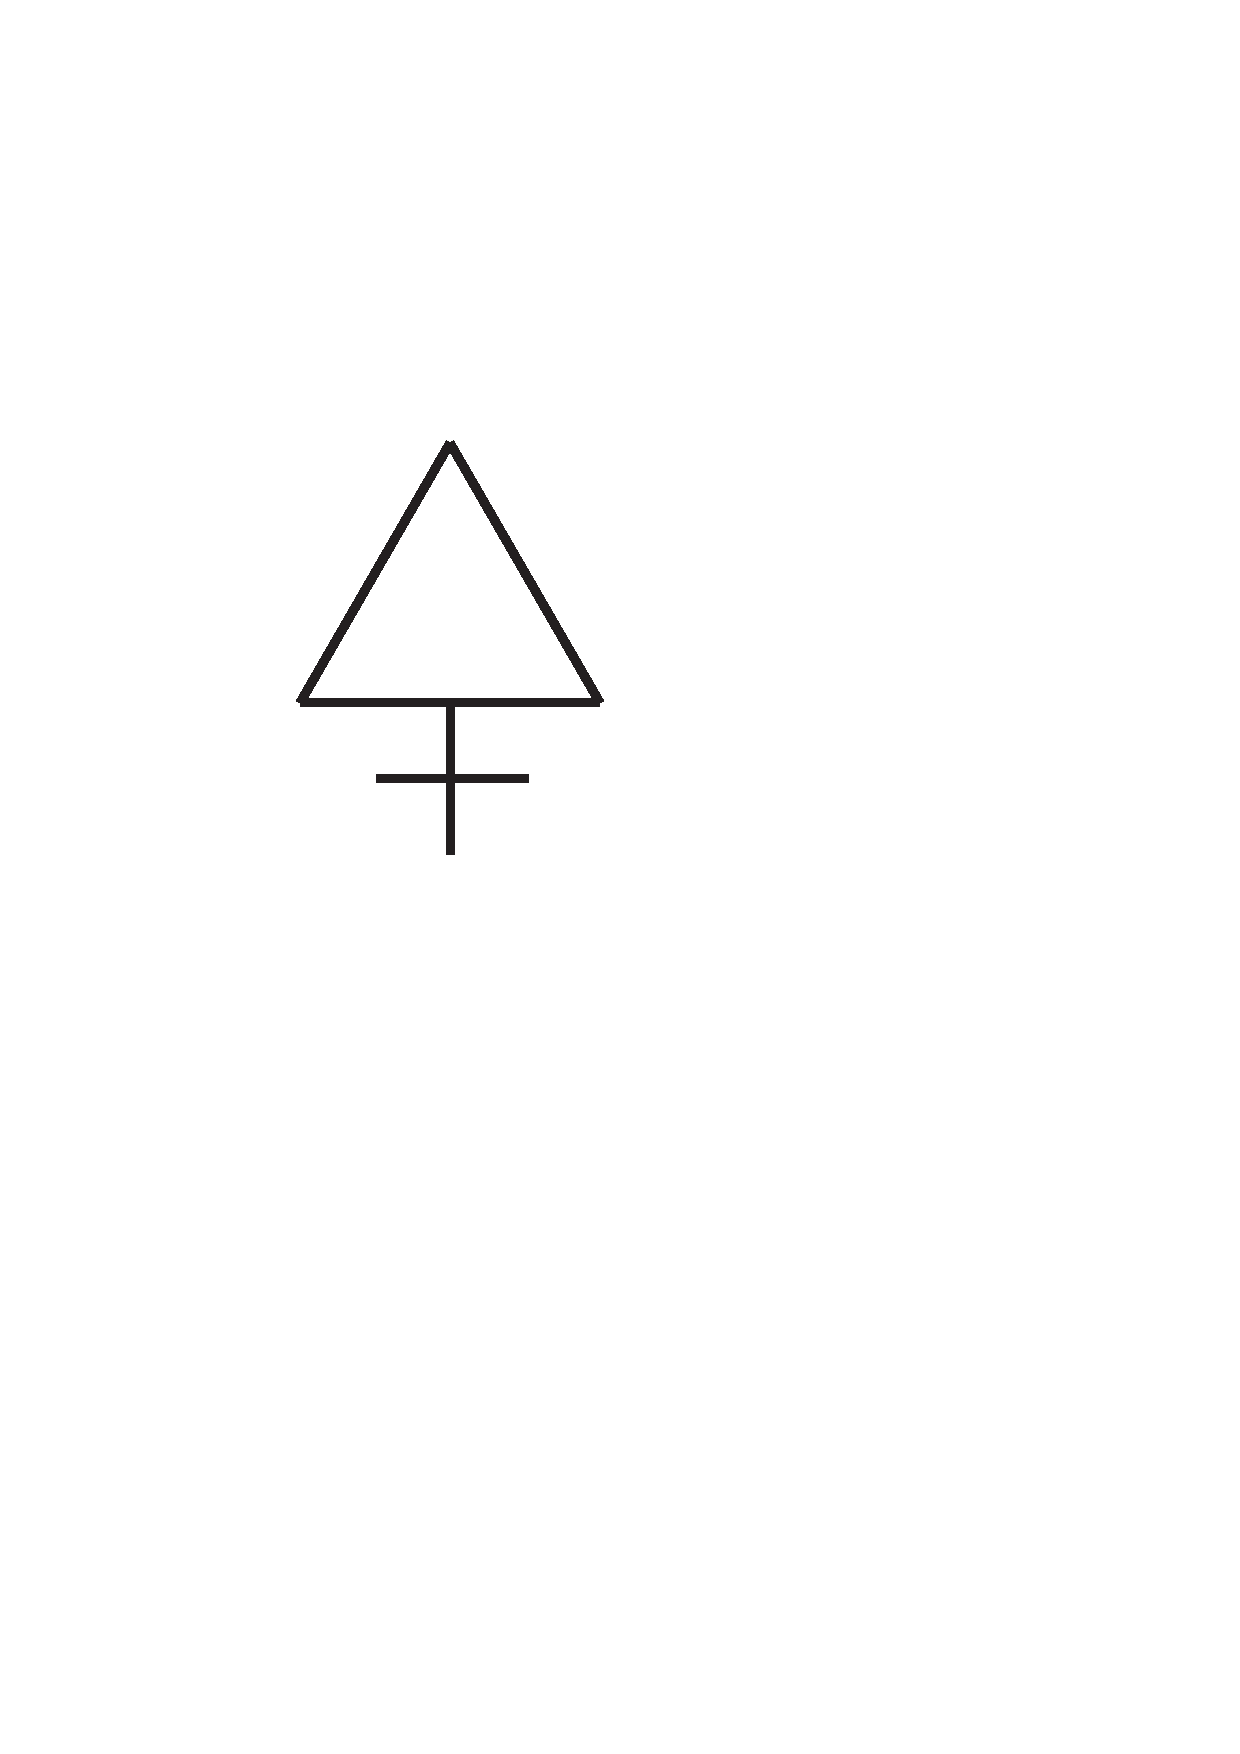
\includegraphics[width=0.02\textwidth]{images/sym-sulph.pdf} & Schwefel\\
%$\rightmoon$ & Silber (Mond)\\
% \protect
\includegraphics[width=0.02\textwidth]{images/taros.pdf} & Tartar\\
%\protect
\includegraphics[width=0.02\textwidth]{images/vitriol.pdf} & Vitriol\\
%$\bigtriangleup$ & Wasser\\
%\protect
\includegraphics[width=0.02\textwidth]{images/sym-spirvini.pdf} & Weingeist (Spiritus vini)\\
%\protect
\includegraphics[width=0.02\textwidth]{images/taros.pdf} & Weinstein (Tartar)\\
%\jupiter & Zinn (Jupiter)
\end{longtable}
\vspace{2.0ex}
%%%%
%%%%
%\newpage

\noindent\footnotesize{\uppercase{5. Mathematische Zeichen}}
\setlength\LTleft{0pt} \setlength\LTright{0pt}
\begin{longtable}{lp{100mm}}
\footnotesize\vspace*{1mm}
$\smallfrown$ & Multiplikation\\\vspace*{1mm}
$\smallsmile$ & Division\\\vspace*{1mm}
$\bigtriangledown$ & Dreieck\\\vspace*{1mm}%
%\rule{1pt}{3mm} & Kürzung eines Bruchs\\\vspace*{1mm}
$f$ & facit\\\vspace*{1mm}
$\square$ \fbox{2} & Quadrat\\\vspace*{1mm}
\fbox{3}~~cub. & Kubus\\\vspace*{1mm}
$\surd~~~\sqrt{~~~}$\ \ Rq. & Quadratwurzel\\\vspace*{1mm}
=\ aequ.\ aeq.\ $\sqcap$ $\rightpropto$ $\squaredots$ & gleich\\ 
$\groesser$ & grö{\ss}er als\\
$\kleiner$ & kleiner als\\ \vspace*{1mm}
%$\infty$ & unendlich\\
, ,, ,,, $\llcorner \lrcorner$ & Klammerausdrücke\\\vspace*{1mm}
\ovalbox{\makebox[15mm][l]{~~~}} & Umrahmungen zur Bezeichnung wegfallender Terme\\\vspace*{1mm}
... ,,, & Platzhalter für Terme\\
$\pleibdashv$ & kombinierte Plusminuszeichen% $+-$ % auch $\pPsMs$\ 
\\
$\pleibvdash$% & kombinierte Vorzeichen $-+$ % auch $\pMsPs$\
\\
$\ppmG$
\\
$\ppmH$ % & kombinierte Vorzeichen $+(-+)$ % auch $\pPsMsPs$\  
\\
$\ppmD$ % & kombinierte Vorzeichen $-(++)$
\\
$\ppmB$ 
%\\
%$\pPsPsMs$\ $\ppmE$\ $\ppmG$% & kombinierte Vorzeichen $+(+-)$ 
%\\
%$\pMsPsMs$%\ & kombinierte Vorzeichen ??$-(+-)$ % oder: plus minus plus ??
%\\
%$\pMsMsPs$%\ & kombinierte Vorzeichen ??$-(-+)$ % oder: minus plus plus ??
%\\
%$\pMsPsPs$\ 
\end{longtable}
\vspace{2.0ex}
%%%%
%%%%

%\noindent\footnotesize{\uppercase{6. Zeichen von Masseinheiten}}
%\setlength\LTleft{0pt} \setlength\LTright{0pt}
%\begin{longtable}{lp{100mm}}
%\footnotesize\vspace*{1mm}
%\protect
\includegraphics[width=0.011\textwidth]{images/drachma.pdf} & Drachme\\
%\protect
\includegraphics[width=0.022\textwidth]{images/semidrachma.pdf} & halbe Drachme\\\vspace*{1mm}
%\protect
\includegraphics[width=0.023\textwidth]{images/semiuncia.pdf} & halbe Unze\\
%\Pfund & Pfund\\\vspace*{1,2mm}
%\protect
\includegraphics[width=0.018\textwidth]{images/sym-scrupulus.pdf} & Skrupel\\
%\protect
\includegraphics[width=0.011\textwidth]{images/uncia.pdf} & Unze
%\end{longtable}
%\vspace{2.0ex}
%%%%
%%%%

%\noindent\footnotesize{\uppercase{7. Sonstige Zeichen}}
%\setlength\LTleft{0pt} \setlength\LTright{0pt}
%\begin{longtable}{lp{100mm}}
%\footnotesize
%\Denarius & destilletur, distilletur (noch zu bedenken)\\
%\textrecipe & recipe (Rezeptur)
%\end{longtable}
%\vspace{2.0ex}
%%%%
%%%%


% \newpage
% \vspace*{4.0ex}% PR: Rein provisorisch!
% \renewcommand*{\chapter}{\OrigChapter}


% \noindent\normalsize{\uppercase{Sonderzeichen für Herrn Bayuk}}\vspace*{3mm}
% \setlength\LTleft{0pt} \setlength\LTright{0pt}
% \begin{longtable}{lp{100mm}}
% \normalsize\vspace*{3mm}
% $\pmA$\ $\ppmA$ & \textit{Bedeutung:} $-(-+)$ \ \textit{Befehl:} $\backslash$pmA \textit{bzw.} $\backslash$ppmA \textit{(gesenkt)}\\
% $\pmB$\ $\ppmB$ & \textit{Bedeutung:} $-(+-)$ \ \textit{Befehl:} $\backslash$pmB \textit{bzw.} $\backslash$ppmB \textit{(gesenkt)}
% \end{longtable}
% \vspace{2.0ex}
%%%%
%%%%
